\usetikzlibrary{arrows.meta}
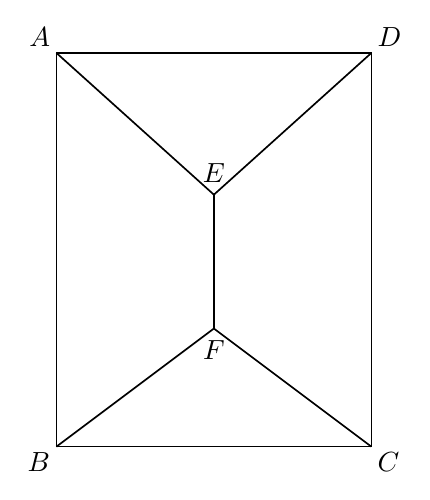
\begin{tikzpicture}[x=1cm,y=1cm,line width=.6pt,font=\normalsize,
  ptlabel/.style={inner sep=0pt}]
% Outer rectangle A(0,5) D(4,5) C(4,0) B(0,0); interior E(2,3.2) F(2,1.5).
\coordinate (A) at (0,5);
\coordinate (D) at (4,5);
\coordinate (C) at (4,0);
\coordinate (B) at (0,0);
\coordinate (E) at (2,3.2);
\coordinate (F) at (2,1.5);
% Outer frame.
\draw (A) -- (D) -- (C) -- (B) -- cycle;
% Interior segments: A-E, D-E, E-F vertical, B-F, C-F.
\draw (A) -- (E);
\draw (D) -- (E);
\draw (E) -- (F);
\draw (B) -- (F);
\draw (C) -- (F);
% Corner labels placed diagonally outward, clear of strokes.
\node[ptlabel,above left,xshift=-2pt,yshift=2pt] at (A) {$A$};
\node[ptlabel,above right,xshift=2pt,yshift=2pt] at (D) {$D$};
\node[ptlabel,below left,xshift=-2pt,yshift=-2pt] at (B) {$B$};
\node[ptlabel,below right,xshift=2pt,yshift=-2pt] at (C) {$C$};
% E label above vertex in wedge between A-E and D-E, 4pt clear.
\node[ptlabel,anchor=south,yshift=4pt] at (E) {$E$};
% F label below vertex in wedge interior of triangle BFC, 4pt clear.
\node[ptlabel,anchor=north,yshift=-4pt] at (F) {$F$};
\end{tikzpicture}
